\documentclass[10pt, twoside]{article}   	% use "amsart" instead of "article" for AMSLaTeX format
\usepackage{geometry}                		% See geometry.pdf to learn the layout options. There are lots.
\geometry{a4paper}                   		% ... or a4paper or a5paper or ... 
\linespread{1.0}
%\geometry{landscape}                		% Activate for rotated page geometry
%\usepackage[parfill]{parskip}    		% Activate to begin paragraphs with an empty line rather than an indent
\usepackage{graphicx}				% Use pdf, png, jpg, or eps§ with pdflatex; use eps in DVI mode
								% TeX will automatically convert eps --> pdf in pdflatex		

\pagestyle{headings}

%SetFonts

\usepackage{mathrsfs}
\usepackage{amsthm,amsmath,amssymb}

%\usepackage{fourier}
%\usepackage{newpxmath}
\usepackage{fontspec}
%\setmainfont{Scala}
%\setmonofont{SF Mono}
\usepackage{xeCJK}
\usepackage{bm}
\usepackage{bbold}

\def\rcurs{{\mbox{$\resizebox{.16in}{.08in}{\includegraphics{ScriptR}}$}}}
\def\brcurs{{\mbox{$\resizebox{.16in}{.08in}{\includegraphics{BoldR}}$}}}
\def\hrcurs{{\mbox{$\hat \brcurs$}}}

\usepackage{color,xcolor}
\usepackage{ebezier}
\usepackage{tikz}
\usepackage{circuitikz}
\usepackage{physics}

\usepackage[colorlinks,
linkcolor = blue,
anchorcolor = blue,
citecolor = blue,
urlcolor = blue]{hyperref}

\usepackage{multirow}
\usepackage{multicol}
\usepackage{makecell}
\usepackage{wrapfig}
\usepackage{caption}

\usepackage{appendix}
\theoremstyle{plain}
\newtheorem{lemma}{Lemma}[section]
\newtheorem{theorem}[lemma]{Theorem}
\newtheorem{axiom}[lemma]{Axiom}
\newtheorem{corollary}[lemma]{Corollary}
\newtheorem{proposition}[lemma]{Proposition}
\theoremstyle{definition}
\newtheorem{definition}[lemma]{Definition}
\newtheorem{remark}{Remark}[section]
\newtheorem{example}[lemma]{Example}

\usepackage{syntonly}
%\syntaxonly

\title{A Cylindrical Lens}
\author{黄远墨~~2023141220092}
\date{}							% Activate to display a given date or no date

\begin{document}
	% generates the title
	\maketitle
	% insert the table of contents
%	\tableofcontents
	
	Mark every parallel ray with its position $x$. For every ray, their optical path length should
	be equal. That is,
	\begin{equation}\label{eqLength}
		C = \sqrt{f^2 + \left(\tfrac{L}{2}\right)^2} = nh + \sqrt{(f - h(x))^2 + x^2},
	\end{equation}
	where $h(x)$ is the thickness of the lens at point $x$. We can rewrite equation
	\eqref{eqLength} as
	\begin{equation}
	h(x) = \frac{nC - f}{n^2 - 1} - \sqrt{\left(\frac{nC - f}{n^2 - 1}\right)^2 - \frac{\left(
	\frac{L}{2}\right)^2 - x^2}{n^2 - 1}}.
	\end{equation}
	We took a reasonable solution where $h(\pm L / 2) = 0$. Then $h(0)$ is easily obtained.

	In fact, $h(x)$ is a branch of the hyperbola
	\begin{equation}
		\frac{\left(h - \frac{nC - f}{n^2 - 1}\right)^2}{\left(\frac{nC - f}{n^2 - 1}\right)^2 -
		\frac{(L / 2)^2}{n^2 - 1}} - \frac{x^2}{\frac{(nC - f)^2}{n^2 - 1} - \left( \frac{L}{2}
		\right)^2} = 1.
	\end{equation}
	Therefore the radius at $x = 0$ is easily calculated with the result of hyperbolae,
	\begin{equation}
		R = \sqrt{(nC - f)^2 - (n^2 - 1)(L / 2)^2}.
	\end{equation}

	\begin{figure}[htbp]
		\centering
		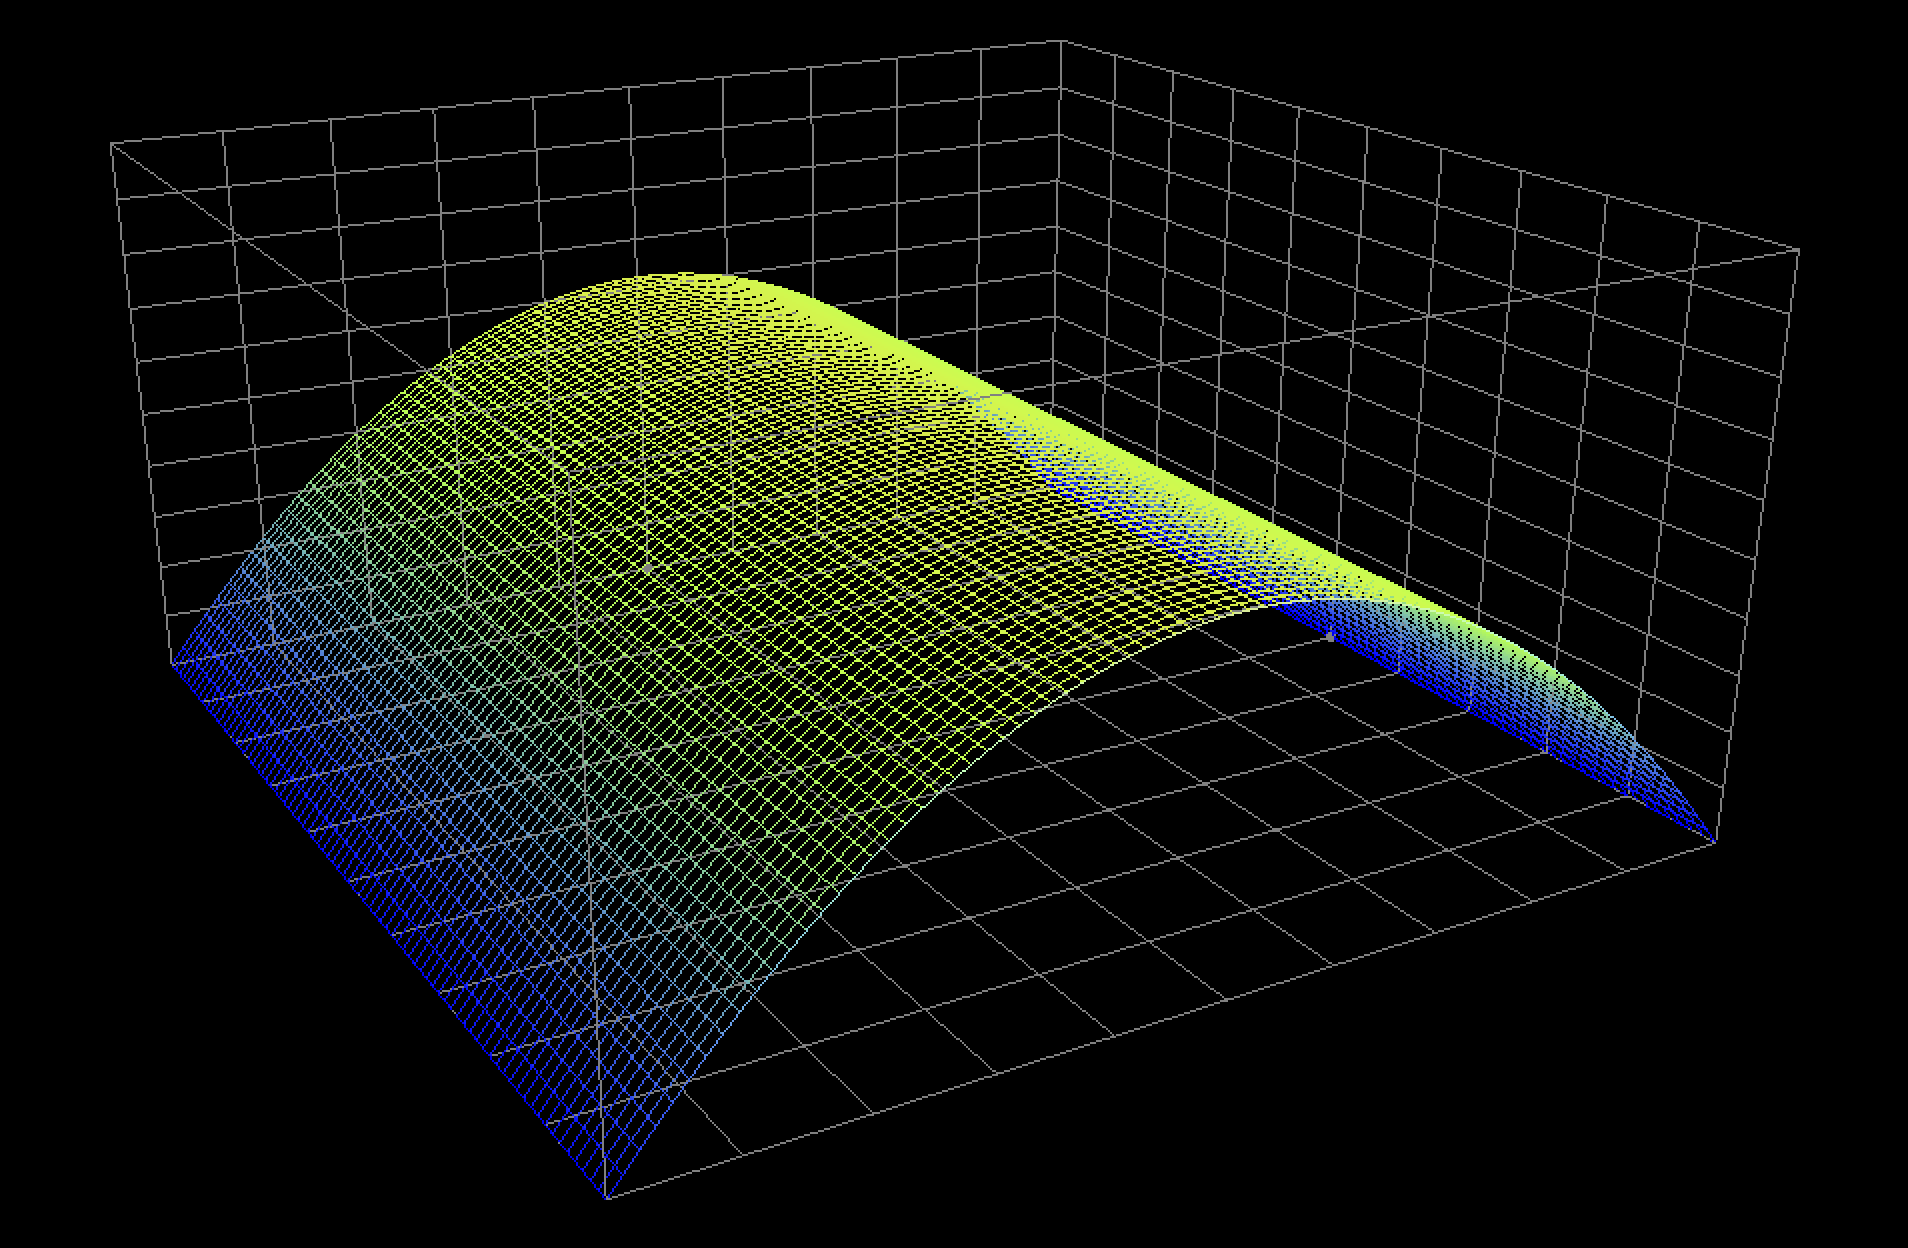
\includegraphics[width=0.7\textwidth]{Surface.png}
		\captionsetup{font={small}}
		\caption{Surface of the lens. $L = 100$, $f = 400$. Height $h(0) = 6.225775$, radius at
		$x = 0$ is $196.8871$.}
	\end{figure}
	
\end{document}


